\chapter{Revisão Bibliográfica}

\section{Considerações Iniciais}

O estudo de Redes Complexas é a base para a compreensão da complexidade, buscando explicar a emergência e 
evolução estrutural do esqueleto de um sistema complexo \cite{barabasi2007architecture}. O estudo da rede
muitas vezes ignora dados mais completos e se atém apenas à presença de conexões entre os nós, o que permite
analisar a estrutura onde os processos ocorrem, fornecendo informações para explicar como comportamentos
emergem de partes mais simples.

\section{Métricas}

Métricas são uma maneira de sumarizar informações necessárias para caracterizar a estrutura de uma rede.
A descrição quantitativa das propriedades de redes fornecem ferramentas fundamentais para a análise de
redes reais e teóricas, permitindo sua representação, caracterização, classificação e modelagem 
\cite{costa2007characterization}.

Nas métricas a seguir supomos que o grafo com $N$ vértices é representado por uma matriz $A \in \mathbb{R}^{N \times N}$, 
onde $A_{ij}$ é 1 caso exista uma aresta entre os vértices $V_i$ e $V_j$, e 0 caso contrário. Grafos não-direcionados 
necessariamente são representados por uma matriz simétrica. Supomos também que o grafo não permite auto-adjacência, isto é, 
$A_{ii} = 0, \forall i$. O número de arestas $M$ pode ser calculado por $\frac{1}{2} \sum A_{ij}$ para grafos 
não-direcionados e por $\sum A_{ij}$ para grafos direcionados. 

Um ponto de interesse é a análise de \emph{distribuições de métricas}, onde
é a cada vértice é associada uma 
medida, e analisamos o histograma destas medidas como amostras de uma distribuição aleatória. ...

\subsection{Distribuição de grau}

O \emph{grau} $k_i$ de um vértice $V_i$ é o número de arestas que contém tal vértice. Em grafos não-direcionados 
calculamos o grau pela Equação \ref{eq:deg-undirected}. Em grafos direcionados podemos também medir 
o número de arestas de entrade e de saída, representadas respectivamente por $k^{in}_i$ e $k^{out}_i$, 
dadas pela equação \ref{eq:deg-directed}. 

\begin{alignat}{4}
 k_i &= \sum_{j} A_{ij}      &\quad          &                  &\quad           &                  &\quad \text{Grafos não-direcionados}\label{eq:deg-undirected} \\
 k_i &= k_i^{out} + k_i^{in} &\quad k_i^{in} &= \sum_{j} A_{ji} &\quad k_i^{out} &= \sum_{j} A_{ij} &\quad \text{Grafos direcionados}\label{eq:deg-directed}
\end{alignat}

O \emph{grau médio} $\langle k \rangle$ de uma rede é a média de graus para todos os vértices, como calculado
na equação \ref{eq:deg-average}. Tal medida é fundamental para muitos modelos.

\begin{equation}
 \langle k \rangle = \frac{1}{N} \sum_{i} k_i = \frac{M}{N}
 \label{eq:deg-average}
\end{equation}

A análise da \emph{distribuição de graus} é uma informação importante sobre uma rede, fornecendo muita informação 
sobre sua estrutura e o comportamento de processos sobre ela. Em específico, no processo de disseminação de informações,
a existência de um limiar de infecção depende da presença do segundo momento da distribuição; 
para redes com variância infinita, este limiar é zero, indicando que a disseminação não pode ser contida uma vez iniciada
em tais redes.

Uma distribuição \emph{exponencial} implica que o grau médio $\langle k \rangle$ é o grau típico da rede, com a 
ocorrência de vértices com grau muito maior ou muito menor exponencialmente raras. Redes com distribuição de grau 
do tipo Poisson (Equação \ref{eq:deg-poisson}) são consideradas redes exponenciais.

Uma distribuição \emph{livre de escala} implica que não existe um grau típico da rede, podendo ocorrer poucos vértices 
com grau muito acima da média. O principal tipo de distribuição é \emph{de Pareto} ou \emph{Lei de Potência}, 
dado pela Equação \ref{eq:deg-pareto}, e redes reais possuem coeficiente $\gamma$ entre 2 e 3 \cite{costa2007characterization}. 
Uma propriedade interessante deste tipo de distribuição é que o número de momentos definidos $m$ obedece 
$m < \gamma-1$. Deste modo, com $\gamma < 3$, a variância é infinita e apenas a média pode ser definida. 
Observe-se que isto é válido para a distribuição teórica; os graus da rede são amostras de uma tal distribuição, 
e sendo em número finito, permitem calcular até $N$ momentos.

\begin{align}
 P(k; \langle k \rangle) &\sim \frac{{\langle k \rangle}^k e^{-\langle k \rangle}}{k!} \label{eq:deg-poisson} \\
 P(k; \gamma) &\sim k^{-\gamma} \label{eq:deg-pareto}
\end{align}

\subsection{Distribuição de \textit{clustering}}

Redes reais, especialmente redes sociais, possuem um número grande de laços pequenos e subconjuntos de vértices 
altamente interconectados. Esta propriedade é chamada de \textit{clustering} (do inglês, ``aglomeração''),
propriedade que está relacionada (mas não limitada) à ocorrência de comunidades. As métricas seguintes 
são definidas apenas para grafos não-direcionados.

A \emph{transitividade} é uma medida da densidade de triângulos (isto é, laços de comprimento 3)
na rede, definida na Equação \ref{eq:transitivity}. $N_3$ é o número de triplas, enquanto $N_\bigtriangleup$
é o número de triplas fechadas. Esta métrica dá um peso igual para cada triângulo, sem distinção sobre quais 
vértices ele contém.

\begin{align}
 C &= \frac{3 N_\bigtriangleup}{N_3} \label{eq:transitivity} \\
 N_\bigtriangleup &= \sum_{k > j > i} A_{ij} A_{jk} A_{ki} \nonumber \\
 N_3 &= \sum_{k > j > i} (A_{ij} A_{ik} + A_{ji} A_{jk} + A_{ki} A_{kj}) \nonumber
\end{align}

O \emph{coeficiente de aglomeração local} $C_i$ mede o \textit{clustering} para cada vértice,
considerando apenas informação dos vértices próximos. Ele é calculado pela Equação \ref{eq:local-clustering}, onde $l_i$
é o número de arestas entre os vizinhos de $V_i$, e $k_i (k_i - 1)$ é o número de arestas
possíveis entre os vizinhos de $V_i$. Em outras palavras, esta medida fornece o quão completo é o subgrafo 
que contém os vizinhos de $V_i$.

\begin{align}
 C_i &= \frac{2 l_i}{k_i (k_i - 1)} \label{eq:local-clustering} \\
 l_i &= \sum_{k > j} A_{ij} A_{jk} A_{ki} \nonumber
\end{align}

A média dos coeficientes de aglomeração locais $\langle C \rangle$ é um resumo da distribuição completa, 
e não deve ser confundida com a transitividade $C$: a primeira dá peso igual para cada vértice, 
enquanto a segunda dá peso igual para cada triângulo.

A aglomeração de uma rede tem impacto sobre a velocidade de disseminação de uma difusão. Dados $I$ nós
infectados, uma primeira análise espera que existam $\langle k \rangle I$ vizinhos imediatos que podem
ser infectados na sequência. Contudo, isto é verdade apenas com baixa aglomeração: para uma alta 
aglomeração espera-se que muitos dos vizinhos sejam compartilhados, diminuindo a quantidade de próximos
infectados possíveis e, por consequência, a velocidade de disseminação.

\subsection{Assortatividade}

Redes de mundo real frequentemente apresentam tipos diferentes de vértices, e a probabilidade de conexão 
entre vértices depende destes tipos \cite{newman2003structure}. Quando nós em uma rede tendem a se
conectar com nós semelhantes a rede é dita \emph{assortativa}; do contrário, é dita \emph{desassortativa}. 

Um caso especial de análise de assortatividade é definir o tipo de um vértice com base no seu 
grau. Seja $k_{nn}(i)$ a média do grau dos vizinhos (\textit{nearest neighbors}) do vértice $V_i$, 
calculado pela Equação \ref{eq:deg-avg-degree}. A assortatividade $r$ de uma rede é definida como o 
coeficiente de Pearson da distribuição das variáveis $k$ e $k_{nn}$ \cite{newman2002assortative}, 
com valor positivo para redes assortativas e negativo para redes desassortativas. 
A Equação \ref{eq:pearson} mostra um procedimento de cálculo de $r$, onde $\langle \cdot \rangle$ 
denota a média e $\sigma(\cdot)$ denota o desvio padrão da distribuição.

\begin{align}
 k_{nn}(i) &= \frac{1}{k_i} \sum_j A_{ij} k_j \label{eq:deg-avg-degree} \\
 r        &= \sum_i \left( \frac{k_i - \langle k \rangle}{\sigma(k)} \right) 
                    \left( \frac{k_{nn}(i) - \langle k_{nn} \rangle}{\sigma(k_{nn})} \right)
             \label{eq:pearson}
\end{align}

Redes assortativas tendem a ser mais resilientes a ataques direcionados, de modo que se alguns 
\textit{hubs} tornarem-se refratários à disseminação (por exemplo, no estado Removido do modelo
SIR), a disseminação persiste se outros \textit{hubs} se mantiverem infecciosos. Do contrário,
redes desassortativas tendem a se tornarem desconectadas quando alguns \textit{hubs} são 
removidos, de modo que a infecção pode falhar em atingir todos os indivíduos.

\subsection{\textit{$K$-Core}}

Algumas redes tendem a se organizar em camadas, onde o núcleo consiste em um conjunto altamente interconectado
de vértices e camadas sucessivas apresentam menor interconexão. A métrica \textit{$k$-core} determina estas 
camadas definindo como núcleo $k$ o maior subgrafo conectado que contém apenas vértices com grau $k$
ou maior. Um vértice no núcleo $k$ também está incluído no núcleo $k-1$, e seu valor de \textit{coreness}
é definido como o maior núcleo ao qual ele pertence.

É possível determinar um núcleo $k$ com um algoritmo $\mathcal{O}(N)$, removendo repetidamente todo vértice
com grau menor que $k$; todos os vértices remanescentes têm \textit{coreness} $k$. Disseminações que se 
iniciam no núcleo central da rede - isto é, em algum vértice com maior \textit{coreness} - afetam um número 
maior de vértices do que se iniciarem em nós com grau equivalente, mas em camadas mais periféricas 
\cite{stanley2010identification}.

\section{Modelos de rede}
\label{sec:modelos}

\subsection{Modelo Erdös-Rényi}

O modelo de redes proposto por Erdős e Rényi \cite{erd6s1960evolution} consiste no modelo de redes aleatórias. Para a criação de uma rede aleatória, imaginemos $n$ vértices, todos desconectados. A cada iteração $m$ escolhe-se um par de vértices aleatoriamente para serem conectados. Nota-se que quanto maior o $m$, maiores as chances de selecionar vértices já conectados, portanto, mais densamente conectado se tornam determinadas áreas de uma rede, evidenciado a geração de \textit{clusters}. Em suma, são adicionadas $m$ arestas de forma aleatória em um número fixo de $n$ vértices.   

Erdős e Rényi estudaram as mudanças na topologia de redes aleatórias em função de $m$. Constatou-se que quanto menor o $m$, as redes tendem a se fragmentar em muitos \textit{clusters} pequenos, os quais são chamados de componentes. À medida que $m$ aumenta, os componentes também aumentam, primeiramente em função de intra-conexões entre vértices isolados de um componentes e posteriormente em função de inter-conexões entre os componentes, como é apresentado na Figura \ref{graph_random}.

\begin{figure}[!htb]
\centering
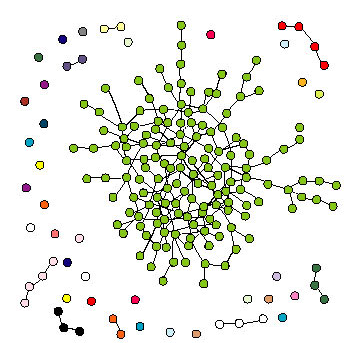
\includegraphics[scale=0.8]{./imagens/graph_random.png}
\caption{Exemplo de rede aleatória \cite{strogatz2001exploring}}
\label{graph_random}
\end{figure}

Desde o trabalho pioneiro, redes aleatórias têm sido estudadas mais profundamente sob o aspecto matemático\cite{bollobas2001random}. A partir deste modelo foram criadas arquiteturas idealizadas para modelos dinâmicos de redes de genes, ecossistemas e a propagação de doenças infecciosas \cite{strogatz2001exploring}. Vale ressaltar que o modelo proposto por Erdős e Rényi abriu porta para pesquisas sobre os demais modelos apresentados nesta seção.

\subsection{Modelo Barabási-Albert}

Redes regulares e aleatórias são ambas boas idealizações e tem suas aplicações no campo da pesquisa \cite{strogatz2001exploring}, porém, a maioria das redes reais tem um padrão intermediário entre a ordem e a desordem. O modelo proposto por Watts e Strogatz \cite{watts1998collective}, denominado rede de Pequeno-Mundo, é capaz de ajustar este meio-termo a partir de uma rede regular. O nome “Pequeno-Mundo”, faz referência ao trabalho de \cite{milgram1967small}, no qual constatou-se que, sob o ponto de vista matemático, quaisquer duas pessoas nos \textbf{Estados Unidos} estão separadas por 5 conhecidos. \cite{guare1992six}, popularizou o termo “Pequeno-Mundo” como “Seis Graus de Separação” em seu livro, considerando a premissa existencial de que quaisquer duas pessoas no \textbf{mundo} estão conectadas por não mais do que 6 conhecidos.

Na interpolação entre redes regulares e randômicas, é considerado o processo de religação randômica apresentado na Figura \ref{graph_world}. Considerando um rede com a estrutura em anel contendo $n$ vértices e $k$ arestas por vértice, percorre-se todas as arestas da rede, religando-as de forma aleatória segundo uma probabilidade $p$. Se $p = 0$ a aresta permanecerá intacta, pois não existe probabilidade alguma de religação, caso contrário, se $p = 1$, a aresta evidentemente será religada de forma aleatória na rede, ou seja, a escolha pelo valor de $p$, de forma que $0 < p < 1$ permite variar entre uma rede aleatório e uma rede regular.

\begin{figure}[!htb]
\centering
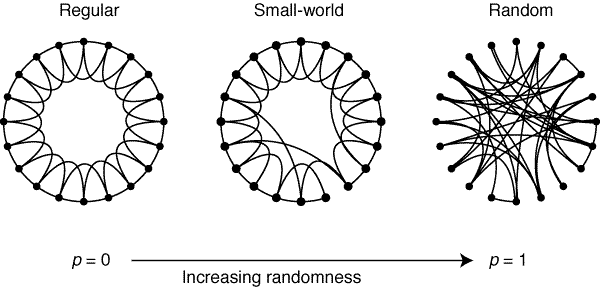
\includegraphics[scale=0.8]{./imagens/graph_world.png}
\caption{Processo de obtenção de uma rede de pequeno-mundo a partir de uma rede regular}
\label{graph_world}
\end{figure}
 
As redes de pequeno mundo apresentam duas propriedades muito importantes \cite{strogatz2001exploring}: (1) Rede altamente agrupadas – Estas redes são muito mais agrupadas do que redes aleatórias. Considerando os \textit{clusters} A, B e C, se A está ligado a B e B está ligado a C, então existe grande probabilidade de A estar conectado a C; e (2) Caminhos geodésicos - A maiores dos vértices estão conectados através de um caminho mínimo (caminho com o menor número de arestas entre um vértice de origem e um vértice destino). O comportamento com relação aos caminhos geodésicos pode ser constatado através da Equação \ref{caminho}, que consiste no cálculo do caminho mínimo médio entre pares de vértices em um grafo não-direcionado, onde $d_{ij}$ é a distância geodésica entre o vértice $i$ e o vértice $j$

\begin{equation}
  L = \frac{1}{\frac{1}{2} n(n+1)} \sum_{i \geq j}d_{ij}\\
  \label{caminho}
\end{equation}

Matematicamente, estas propriedades podem ser evidenciadas com cálculos estatísticos. Primeiramente vale ressaltar que para que as propriedades sejam válidas assume-se que o grafo não possui vértices desconexos, isso implica em $n > k > ln(n) > 1$, no qual $k > ln(n)$ garante que um grafo aleatório será conectado. Sendo $L(p)$ o caminho mínimo médio (\ref{caminho}) e $C(p)$ o coeficiente de agrupamento médio (\ref{clustering}), tal que $a_i$ é o número de conexões entre os $k_i$ vizinhos do vértice $i$. Nas condições especificadas, quando $p \rightarrow 0$, $L$ TERMINAR.

\begin{equation}
  C = \frac{1}{n} \sum_{i = 1}^{n}\frac{2a_i}{k_i(k_i - 1)}\\
  \label{clustering}
\end{equation}

Watts e Strogatz constataram que estas duas propriedades estão presentes também em muitas redes naturais e tecnológicas \cite{watts1998collective}, como a rede neural da minhoca textit{Caenorhabditis Elegans}, a rede de energia do oeste do Estados Unidos e o grafo de colaboração entre autores em filmes. Além disso, constatou-se que sistemas dinâmicos com os efeitos de pequeno-mundo apresentam aumento na velocidade de propagação do sinal, poder computacional e sincronização. Em geral, os caminhos mínimos provêm canais de comunicação de alta velocidade entre diferentes partes do sistema, facilitando os processos dinâmicos, como sincronização, que requer informação com relação ao estado global do sistema \cite{strogatz2001exploring}. Além disso, doenças infecciosas se espalham mais rapidamente em redes de Pequeno-Mundo.

\subsection{Modelo Watts-Strogatz}

Em redes reais, alguns nós são mais conectados do que outros. No modelo proposto por Barabasi e Albert \cite{barabasi1999emergence}, denominado Livre de Escala, as redes apresentam uma ordem na dinâmica de estruturação. As redes Livres de Escala possuem duas características chave presentes em redes reais: (1) Incorporam crescimento; e (2) Apresentam conexão preferencial. A conexão preferencial se refere a tendência de um novo vértice conectar-se a um vértice de grau elevado. Estes nós altamente conectados são chamados de \textit{hubs}.

\cite{barabasi1999emergence} afirmam que, independentemente do sistema ou da identidade de seus constituintes, a probabilidade $P(k)$ de que um vértice interaja com $k$ vértices decai como uma Lei de Potência, sendo $P(k) \sim k^{-y}$, ou seja, decai muito mais lentamente que Poisson, distribuição de graus prevista em uma rede aleatória \cite{strogatz2001exploring}. Na Lei de Potência, o expoente $y$ determina a taxa de decaimento, que é tipicamente medida no intervalo $2 < y < 3$. Na rede da internet, a probabilidade de $k$ documentos apontarem para uma certa página da \textit{web} segue a Lei de Potência com $y = 2.1 \pm 0.1$ \cite{barabasi1995emergence}. 

Em outras palavras, uma rede aleatória possui grande parte dos vértices com número de conexões próximo da média da distribuição, de forma que cada aresta está presente ou ausente com probabilidade igual. Diferentemente, em redes livres de escala a distribuição do grau dos vértices decai lentamente para a direita, formando uma "cauda", indicando que a maioria dos nós tem grau menor que a média da distribuição \cite{watts2004new}, de forma que a probabilidade da existência de um vértice com grau alto é muito menor do que um vértice com grau baixo. Este comportamento é ilustrado na Figura \ref{comp_distr}.

\begin{figure}[!htb]
\centering
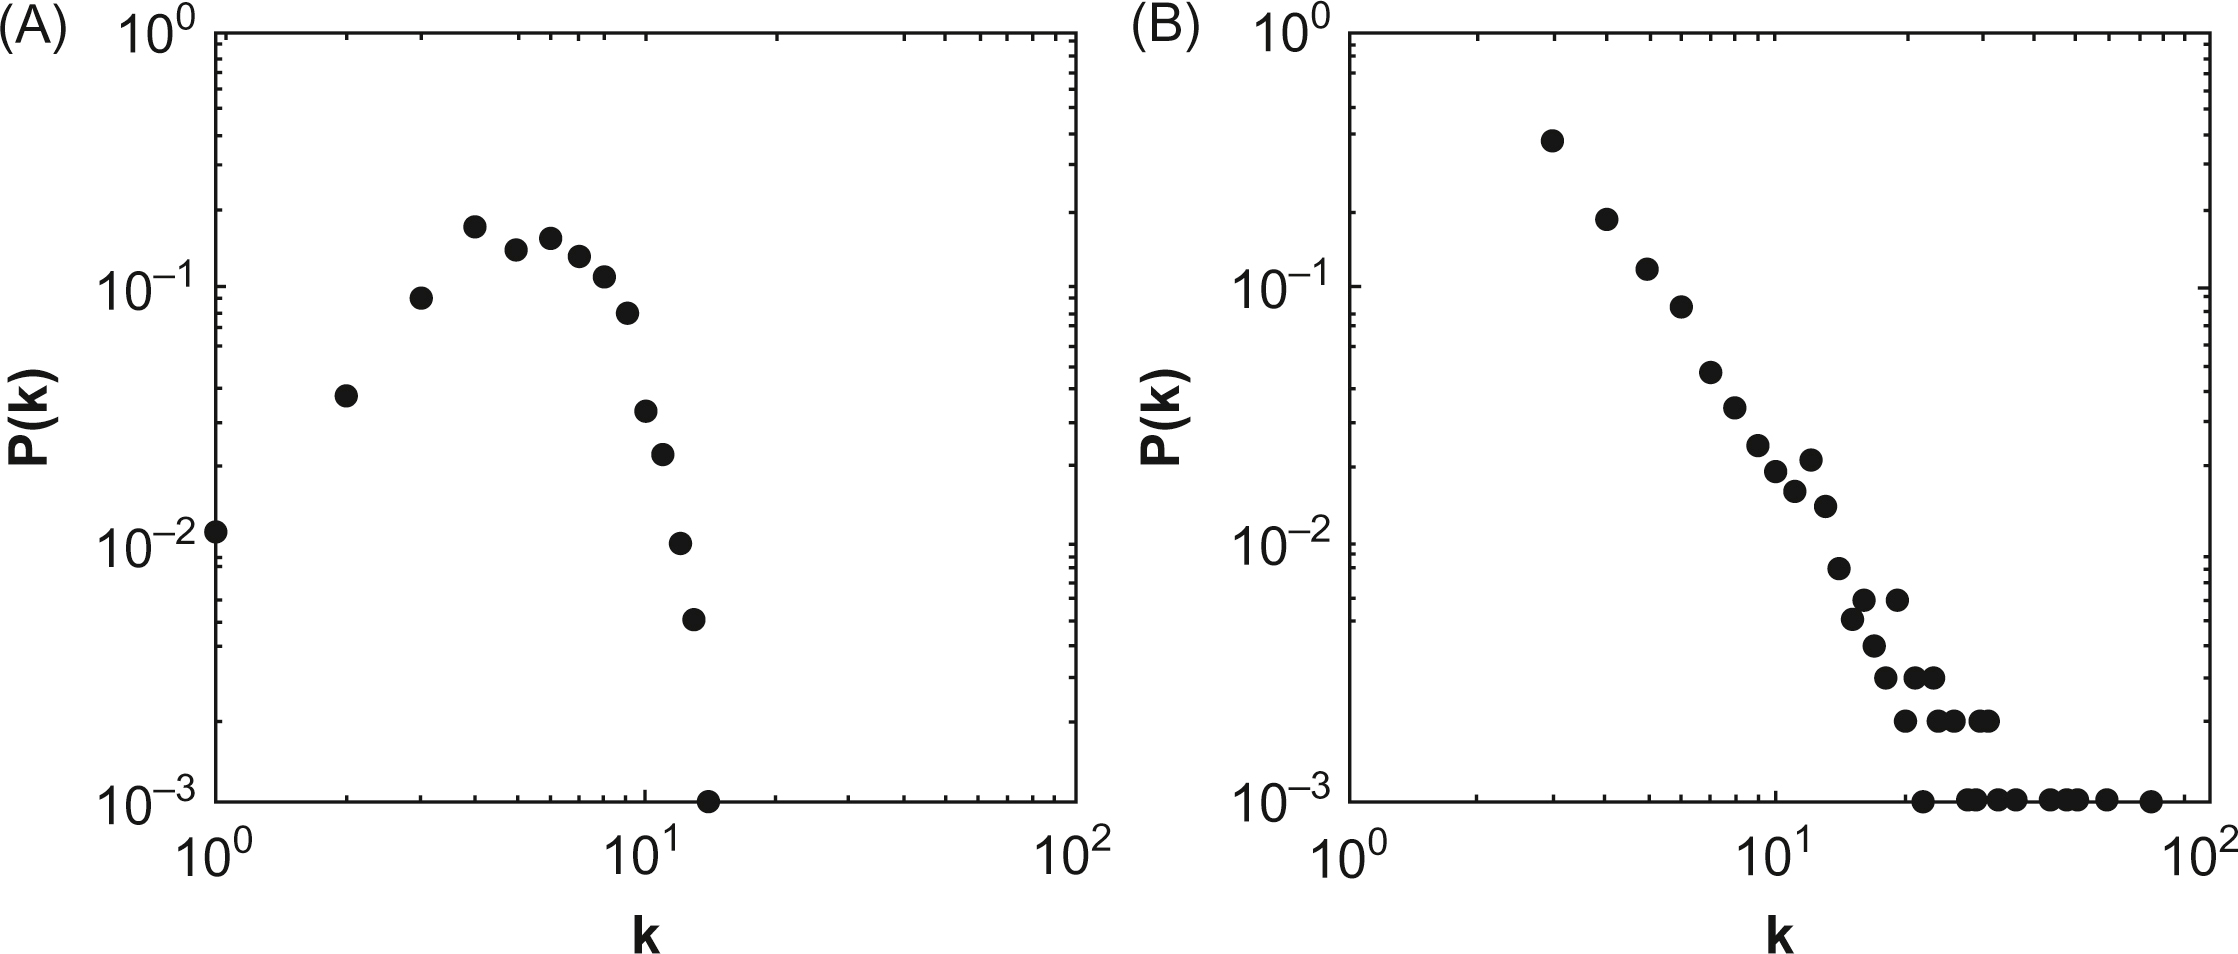
\includegraphics[scale=0.15]{./imagens/comparisson.png}
\caption{Comparação entre a distribuição de uma rede aleatória e uma rede livre de escala cite{scott2011network}}
\label{comp_distr}
\end{figure}

Este comportamento é notado em grande parte das redes reais. No Twitter, pessoas normalmente seguem amigos e pessoas famosas que dispõe informações de sua vida pessoal. Em uma rede de citações de artigos, é evidente que pesquisadores têm preferência em citar trabalhos conhecidos e bem publicados. Um exemplo de uma rede Livre de Escala é apresentado na Figura \ref{graph_scale}

\begin{figure}[!htb]
\centering
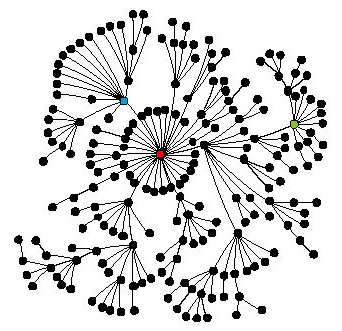
\includegraphics[scale=0.8]{./imagens/scale_free.png}
\caption{Exemplo de rede Livre de Escala} \cite{strogatz2001exploring}
\label{graph_scale}
\end{figure}

\subsection{Modelo Ravasz-Barabási}

Muitas redes reais que modelam fenômenos naturais e sociais possuem duas propriedades genéricas: (1) são livres de escala e (2) apresentam um alto grau de agrupamento. Resultados empíricos mostraram que o coeficiente de agrupamento médio (\ref{clustering}) é significamente maior para redes reais do que para redes aleatórias de mesmo tamanho. Ao mesmo tempo muitas redes científicas e biológicas demonstraram ter a propriedade de serem livres de escala. Modelos propostos para descrever a topologia de redes complexas, em geral tem dificuldade em apresentar tais características simultaneamente.

Ravasz e Barabási \cite{ravasz2003hierarchical} mostraram que estas duas propriedades ocorrem devido a presença de uma organização hierárquica. Portanto, o modelo proposto por \cite{ravasz2003hierarchical} consiste em uma rede que combina a propriedade de redes Livre de Escala e de alto grau de agrupamento.

\begin{figure}[!htb]
\centering
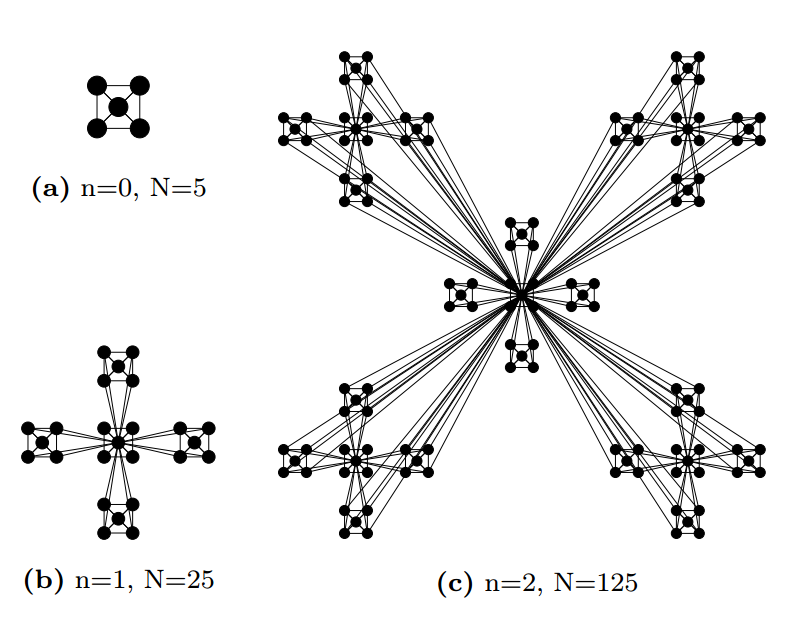
\includegraphics[scale=0.4]{./imagens/graph_h.png}
\caption{Exemplo do processo de formação de uma rede hierárquica \cite{ravasz2003hierarchical}} 
\label{graph_h}
\end{figure}


